\documentclass[aspectratio=43]{beamer}

\makeatletter
\def\input@path{{../../inc/}}
\makeatother
% Pakete für das Dokument

%\usepackage{blindtext}
\graphicspath{{../../assets/images/}}
\usepackage{beamerthememnrstyle}

% Eigenes Theme laden
\usetheme{mnrstyle}

% Eigene Definition von enumerate
% \setlist[enumerate, 2]{label=\roman*., format=\itshape, leftmargin=2cm}

% Metadaten für das Dokument
\title{Glaubensbekenntnis MNR}
\author{OTS}
\date{2025}
\begin{document}
\setmnrTitle{Inhalt}
\begin{frame}
    \begin{center}        
        \begin{enumerate}
            \item \uppercase{Turmbau von Babylon}
            \item \uppercase{Turmbau im volk Gottes}
            \item \uppercase{Turmbau in der Gemeinde}        
            \item \uppercase{Turmbau bei mir}        
        \end{enumerate}
    \end{center}
\end{frame}
\setmnrTitle{Turmbau von Babylon}
\begin{frame}  
    %\begin{mnrframe}
    \vspace*{1cm}
        \begin{exampleblock}{1Mos 11,1 -- 11}
            \color{black}
            \small
            Und die ganze Erde hatte eine einzige Sprache und dieselben Worte.
            Und es geschah, als sie nach Osten zogen, da fanden sie eine Ebene im Land Sinear, und sie ließen sich dort nieder.
            Und sie sprachen zueinander: Wohlan, lasst uns Ziegel streichen und sie feuerfest brennen! Und sie verwendeten Ziegel statt Steine und Asphalt statt Mörtel.
            Und sie sprachen: Wohlan, lasst uns eine Stadt bauen und einen Turm, dessen Spitze bis an den Himmel reicht, dass wir uns einen Namen machen, damit wir ja nicht über die ganze Erde zerstreut werden!            
            Da stieg der HERR herab, um die Stadt und den Turm anzusehen, den die Menschenkinder bauten.
            Und der HERR sprach: Siehe, sie sind ein Volk, und sie sprechen alle eine Sprache, und dies ist [erst] der Anfang ihres Tuns! Und jetzt wird sie nichts davor zurückhalten, das zu tun, was sie sich vorgenommen haben.
            Wohlan, lasst uns hinabsteigen und dort ihre Sprache verwirren, damit keiner mehr die Sprache des anderen versteht!
            So zerstreute der HERR sie von dort über die ganze Erde, und sie hörten auf, die Stadt zu bauen.
            Daher gab man ihr den Namen Babel, weil der HERR dort die Sprache der ganzen Erde verwirrte und sie von dort über die ganze Erde zerstreute.  
        \end{exampleblock}  
    \vspace*{1cm}
    %\end{mnrframe}
\end{frame}
\begin{frame}  
    %\begin{mnrframe}
    \vspace*{1cm}
        \begin{exampleblock}{1Mos 11,1 -- 11}
            \color{black}
            \small
            \begin{greenblock}
                \textbf{1 Und die ganze Erde hatte eine einzige Sprache und dieselben Worte.}
            \end{greenblock}
            Und es geschah, als sie nach Osten zogen, da fanden sie eine Ebene im Land Sinear, und sie ließen sich dort nieder.
            Und sie sprachen zueinander: Wohlan, lasst uns Ziegel streichen und sie feuerfest brennen! Und sie verwendeten Ziegel statt Steine und Asphalt statt Mörtel.
            Und sie sprachen: Wohlan, lasst uns eine Stadt bauen und einen Turm, dessen Spitze bis an den Himmel reicht, dass wir uns einen Namen machen, damit wir ja nicht über die ganze Erde zerstreut werden!            
            Da stieg der HERR herab, um die Stadt und den Turm anzusehen, den die Menschenkinder bauten.
            
            Und der HERR sprach: Siehe, sie sind ein Volk, und sie sprechen alle eine Sprache, und dies ist [erst] der Anfang ihres Tuns! Und jetzt wird sie nichts davor zurückhalten, das zu tun, was sie sich vorgenommen haben.
            Wohlan, lasst uns hinabsteigen und dort ihre Sprache verwirren, damit keiner mehr die Sprache des anderen versteht!
            So zerstreute der HERR sie von dort über die ganze Erde, und sie hörten auf, die Stadt zu bauen.
            Daher gab man ihr den Namen Babel, weil der HERR dort die Sprache der ganzen Erde verwirrte und sie von dort über die ganze Erde zerstreute.  
        \end{exampleblock}  
    \vspace*{1cm}
    %\end{mnrframe}
\end{frame}
\begin{frame}  
    %\begin{mnrframe}
    \vspace*{1cm}
        \begin{exampleblock}{1Mos 11,1 -- 11}
            \color{black}
            \small
            Und die ganze Erde hatte eine einzige Sprache und dieselben Worte.
            \begin{greenblock}
                \textbf{2 Und es geschah, als sie nach Osten zogen, da fanden sie eine Ebene im Land Sinear, und sie ließen sich dort nieder.}
            \end{greenblock}            
            Und sie sprachen zueinander: Wohlan, lasst uns Ziegel streichen und sie feuerfest brennen! Und sie verwendeten Ziegel statt Steine und Asphalt statt Mörtel.
            Und sie sprachen: Wohlan, lasst uns eine Stadt bauen und einen Turm, dessen Spitze bis an den Himmel reicht, dass wir uns einen Namen machen, damit wir ja nicht über die ganze Erde zerstreut werden!            
            Da stieg der HERR herab, um die Stadt und den Turm anzusehen, den die Menschenkinder bauten.
            
            Und der HERR sprach: Siehe, sie sind ein Volk, und sie sprechen alle eine Sprache, und dies ist [erst] der Anfang ihres Tuns! Und jetzt wird sie nichts davor zurückhalten, das zu tun, was sie sich vorgenommen haben.
            Wohlan, lasst uns hinabsteigen und dort ihre Sprache verwirren, damit keiner mehr die Sprache des anderen versteht!
            So zerstreute der HERR sie von dort über die ganze Erde, und sie hörten auf, die Stadt zu bauen.
            Daher gab man ihr den Namen Babel, weil der HERR dort die Sprache der ganzen Erde verwirrte und sie von dort über die ganze Erde zerstreute.  
        \end{exampleblock}  
    \vspace*{1cm}
    %\end{mnrframe}
\end{frame}
\begin{frame}
    \vspace{.7cm}
    \begin{figure}[ht]
    
    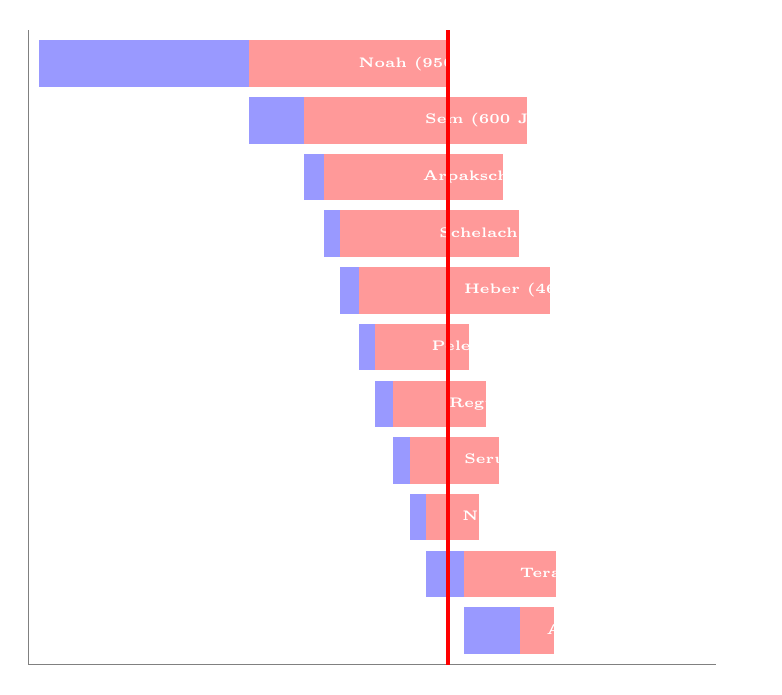
\begin{tikzpicture}[scale=0.8]
    \begin{scope}[scale=0.9]
        \draw[gray] (0,0) -- (0mm, 112mm);
        
        %Noah 500-450 (0 - 93.6)
        \filldraw[blue!40] (2mm,110mm) rectangle(39mm,102mm);
        \filldraw[red!40] (39mm,110mm) rectangle(74.1mm,102mm) node[right, pos=.5, align=left, white] {\tiny \textbf{Noah (950 Jahre)}};
        
        %Sem 100-500 (0 - 93.6)
        \filldraw[blue!40] (39mm, 100mm) rectangle(48.8mm,92mm);
        \filldraw[red!40] (48.8mm,100mm) rectangle(87.8mm,92mm) node[right, pos=.5, align=left, white] {\tiny  \textbf{Sem (600 Jahre)}};
        
         %Arpakschad 35-403 (15.6 - 62.4)
         \filldraw[blue!40] (48.8mm,90mm) rectangle(52.2mm,82mm);
        \filldraw[red!40] (52.2mm,90mm) rectangle(83.6mm,82mm) node[right, pos=.5, align=left, white]  {\tiny \textbf{Arpakschad (438 Jahre)}};
        
        %Schelach 30-403 (15.6 - 62.4)
        \filldraw[blue!40] (52.2mm,80mm) rectangle(55.1mm,72mm);
        \filldraw[red!40] (55.1mm,80mm) rectangle(86.5mm,72mm) node[right, pos=.5, align=left, white] {\tiny \textbf{Schelach (433 Jahre)}};
        
        \filldraw[blue!40] (55.1mm,70mm) rectangle(58.4mm,62mm);
        \filldraw[red!40] (58.4mm,70mm) rectangle(91.9mm,62mm) node[right, pos=.5, align=left, white] {\tiny \textbf{Heber (464 Jahre)}};
        
        \filldraw[blue!40] (58.4mm,60mm) rectangle(61.3mm,52mm);
        \filldraw[red!40] (61.3mm,60mm) rectangle(77.6mm,52mm) node[right, pos=.5, align=left, white] {\tiny \textbf{Peleg (239 Jahre)}};
        
        \filldraw[blue!40] (61.3mm,50mm) rectangle(64.4mm,42mm);
        \filldraw[red!40] (64.4mm,50mm) rectangle(80.6mm,42mm) node[right, pos=.5, align=left, white] {\tiny \textbf{Regu (239 Jahre)}};
        
        \filldraw[blue!40] (64.4mm,40mm) rectangle(67.4mm,32mm);
        \filldraw[red!40] (67.4mm,40mm) rectangle(83.0mm,32mm) node[right, pos=.5, align=left, white] {\tiny \textbf{Serug (230 Jahre)}};
        
        \filldraw[blue!40] (67.4mm,30mm) rectangle(70.2mm,22mm);
        \filldraw[red!40] (70.2mm,30mm) rectangle(79.5mm,22mm) node[right, pos=.5, align=left, white] {\tiny \textbf{Nahor (148 Jahre)}};
        
        \filldraw[blue!40] (70.2mm,20mm) rectangle(77mm,12mm);
        \filldraw[red!40] (77mm,20mm) rectangle(93.0mm,12mm) node[right, pos=.5, align=left, white] {\tiny \textbf{Terach (275 Jahre)}};

        \filldraw[blue!40] (77mm,10mm) rectangle(86.8mm,2mm);
        \filldraw[red!40] (86.8mm,10mm) rectangle(92.6mm,2mm) node[right, pos=.5, align=left, white] {\tiny \textbf{Abraham (175 Jahre)}};
        \draw[gray] (0,0) -- (\textwidth, 0mm);
        \draw[red, line width=.5mm] (74mm,0) -- (74mm, 112mm);
        \end{scope}
    \end{tikzpicture}

    \caption{Lebensjahre von Noah bis Abraham}
    \label{balken_alter}

\end{figure}
\end{frame}
\begin{frame}  
    %\begin{mnrframe}
    \vspace*{1cm}
        \begin{exampleblock}{1Mos 10,9}
            \color{black}            
            Er war ein gewaltiger Jäger vor dem HERRN; daher sagt man: Wie Nimrod, ein gewaltiger Jäger vor dem HERRN!
        \end{exampleblock}  
    \vspace*{1cm}
    %\end{mnrframe}
\end{frame}
\begin{frame}  
    %\begin{mnrframe}
    \vspace*{1cm}
        \begin{exampleblock}{1Mos 10,5.20.31}
            \color{black}            
            Und Gott segnete Noah und seine Söhne und sprach zu ihnen: Seid fruchtbar und vermehrt euch und füllt die Erde!
        \end{exampleblock}  
    \vspace*{1cm}
    %\end{mnrframe}
\end{frame}
\begin{frame}  
    %\begin{mnrframe}
    \vspace*{1cm}
        \begin{exampleblock}{1Mos 9,1}
            \color{black}            
            Das sind die Söhne Hams nach ihren Geschlechter, Sprachen, Ländern und Völkern.
        \end{exampleblock}  
    \vspace*{1cm}
    %\end{mnrframe}
\end{frame}
\setmnrTitle{Turmbau im Volk Israel}
\begin{frame}  
    %\begin{mnrframe}
    \vspace*{1cm}
        \begin{exampleblock}{1Mos 12,1}
            \color{black}            
            Der HERR aber hatte zu Abram gesprochen: Geh hinaus aus deinem Land und aus deiner Verwandtschaft und aus dem Haus deines Vaters in das Land, das ich dir zeigen werde!
        \end{exampleblock}  
    \vspace*{1cm}
    %\end{mnrframe}
\end{frame}
\begin{frame}  
    %\begin{mnrframe}
    \vspace*{1cm}
        \begin{exampleblock}{Ri 8,27}
            \color{black}            
            Und Gideon machte ein Ephod daraus und stellte es in seiner Stadt auf, in Ophra. Und ganz Israel hurte ihm dort nach. Und das wurde zum Fallstrick für Gideon und sein Haus.
        \end{exampleblock}  
    \vspace*{1cm}
    %\end{mnrframe}
\end{frame}
\begin{frame}  
    %\begin{mnrframe}
    \vspace*{1cm}
        \begin{exampleblock}{1. Sam 15,3}
            \color{black}            
            So ziehe nun hin und schlage Amalek und vollstrecke den Bann an allem, was er hat, und schone ihn nicht; sondern töte Männer und Frauen, Kinder und Säuglinge, Rinder und Schafe, Kamele und Esel!
        \end{exampleblock}  
    \vspace*{1cm}
    %\end{mnrframe}
\end{frame}
\begin{frame}  
    %\begin{mnrframe}
    \vspace*{1cm}
        \begin{exampleblock}{1. Sam 15,9}
            \color{black}            
            Aber Saul und das Volk verschonten Agag und die besten Schafe und Rinder und das Vieh vom zweiten Wurf und die Mastschafe und alles, was wertvoll war, und sie wollten den Bann an ihnen nicht vollstrecken; alles Vieh aber, das werlos und schwächlich war, an dem vollstreckten sie den Bann.
        \end{exampleblock}  
    \vspace*{1cm}
    %\end{mnrframe}
\end{frame}
\begin{frame}  
    %\begin{mnrframe}
    \vspace*{1cm}
        \begin{exampleblock}{1. Sam 15,21}
            \color{black}            
            Aber das Volk hat von der Beute genommen, Schafe und Rinder, das Beste des Gebannten, um es dem HERRN, deinem Gott, in Gilgal zu opfern!
        \end{exampleblock}  
    \vspace*{1cm}
    %\end{mnrframe}
\end{frame}
\begin{frame}  
    %\begin{mnrframe}
    \vspace*{1cm}
        \begin{exampleblock}{1. Sam 15,22-23}
            \color{black}            
            Samuel aber sprach: Hat der HERR dasselbe Wohlgefallen an Schlachtopfern und Brandopfern wie daran, dass man der Stimme des HERRN gehorcht? Siehe, Gehorsam ist besser als Schlachtopfer, und Folgsamkeit besser als das Fett von Widdern! Denn Rebellion ist wie die Sünde der Wahrsagerei, und Widerspenstigkeit ist wie Abgötterei und Götzendienst. Weil du das Wort des HERRN verworfen hast, so hat er dich auch verworfen, dass du nicht mehr König sein sollst.
        \end{exampleblock}  
    \vspace*{1cm}
    %\end{mnrframe}
\end{frame}
\begin{frame}  
    %\begin{mnrframe}
    \vspace*{1cm}
        \begin{exampleblock}{2.\,Chr 26,4}
            \color{black}            
            Und er tat, was recht war in den Augen des HERRN, ganz wie es sein Vater Amazja getan hat.
        \end{exampleblock}  
    \vspace*{1cm}
    %\end{mnrframe}
\end{frame}
\begin{frame}  
    %\begin{mnrframe}
    \vspace*{1cm}
        \begin{exampleblock}{2.\,Chr 26,15}
            \color{black}            
            \dots so verbreitete sich sein Ruhm weithin, weil ihm wunderbar geholfen wurde, bis er sehr stark war.
        \end{exampleblock}  
    \vspace*{1cm}
    %\end{mnrframe}
\end{frame}
\begin{frame}  
    %\begin{mnrframe}
    \vspace*{1cm}
        \begin{exampleblock}{2.\,Chr 26,16}
            \color{black}            
            Als er aber stark geworden war, überhob sich sein Herz zu seinem Verderben und er versündigte sich an dem HERRN, seinem Gott, indem er in die Tempelhalle des HERRN ging, um auf dem Räucheraltar zu räuchern.
        \end{exampleblock}  
    \vspace*{1cm}
    %\end{mnrframe}
\end{frame}
\begin{frame}  
    %\begin{mnrframe}
    \vspace*{1cm}
        \begin{exampleblock}{Matt 15,14}
            \color{black}            
            Lasst sie; sie sind blinde Blindenleiter! Wenn aber ein Blinder den anderen leitet, werden beide in die Grube fallen.
        \end{exampleblock}  
    \vspace*{1cm}
    %\end{mnrframe}
\end{frame}
\setmnrTitle{Turmbau der Gemeinde}
\begin{frame}  
    %\begin{mnrframe}
    \vspace*{1cm}
        \begin{exampleblock}{Joh 11,25-26}
            \color{black}            
            Jesus spricht zu ihr: Ich bin die Auferstehung und das Leben. Wer an mich glaubt, wird leben, auch wenn er stribt; und jeder, der lebt und an mich glaubt, wird in Ewigkeit nicht sterben.
        \end{exampleblock}  
        \begin{exampleblock}{Joh 1,12-13}
            \color{black}            
            Allen aber, die ihn aufnahmen, denen gab er das Anrecht, Kinder Gottes zu werden, denen, die an seinen Namen glauben; die nicht aus dem Blut, noch aus dem Willen des Fleisches, noch aus dem Willen des Mannes, sondern aus Gott geboren sind.
        \end{exampleblock}  
        \begin{exampleblock}{Mk 16,15}
            \color{blue}            
            Und er sprach zu ihnen: Geht hin in alle Welt und verkündigt das Evangelium der ganzen Schöpfung.
        \end{exampleblock}  
    \vspace*{1cm}
    %\end{mnrframe}
\end{frame}
\begin{frame}  
    %\begin{mnrframe}
    \vspace*{1cm}
        \begin{exampleblock}{Apg 2,40-41}
            \color{black}            
            Und noch mit vielen anderen Worten gab er Zeugnis und ermahnte und sprach: Lasst euch retten aus diesem verkehrten Geschlecht! Diejenigen, die nun breitwillig sein Wort annahmen, liessen sich taufen, und es wurde an jenem Tag etwa $3000$ Seelen hinzugetan.
        \end{exampleblock}  
    \vspace*{1cm}
    %\end{mnrframe}
\end{frame}
\begin{frame}  
    %\begin{mnrframe}
    \vspace*{1cm}
        \begin{exampleblock}{Gal 5,6}
            \color{black}            
            denn in Christus Jesus gilt weder Beschneidung noch Unbeschnittensein etwas, sondern der Glaube, der durch die Liebe wirksam ist.
        \end{exampleblock}  
    \vspace*{1cm}
    %\end{mnrframe}
\end{frame}
\begin{frame}  
    %\begin{mnrframe}
    \vspace*{1cm}
        \begin{exampleblock}{Joh 11,25-26}
            \color{black}            
            Jesus spricht zu ihr: Ich bin die Auferstehung und das Leben. Wer an mich glaubt, wird leben, auch wenn er stribt; und jeder, der lebt und an mich glaubt, wird in Ewigkeit nicht sterben.
        \end{exampleblock}  
        \begin{exampleblock}{Joh 1,12-13}
            \color{black}            
            Allen aber, die ihn aufnahmen, denen gab er das Anrecht, Kinder Gottes zu werden, denen, die an seinen Namen glauben; die nicht aus dem Blut, noch aus dem Willen des Fleisches, noch aus dem Willen des Mannes, sondern aus Gott geboren sind.
        \end{exampleblock}  
        \begin{exampleblock}{Mk 16,15}
            \color{blue}            
            Und er sprach zu ihnen: Geht hin in alle Welt und verkündigt das Evangelium der ganzen Schöpfung.
        \end{exampleblock}  
    \vspace*{1cm}
    %\end{mnrframe}
\end{frame}
\end{document}